% Graphic for TeX using PGF
% Title: /home/nevj/common/Dia/tradeoff2.dia
% Creator: Dia v0.97.3
% CreationDate: Fri Dec 15 21:15:49 2017
% For: nevj
% \usepackage{tikz}
%\begin{document}
\begin{landscape}
\begin{figure}[!h]
  \centering
\label{fig:tradeoff}

% The following commands are not supported in PSTricks at present
% We define them conditionally, so when they are implemented,
% this pgf file will use them.
\ifx\du\undefined
  \newlength{\du}
\fi
\setlength{\du}{15\unitlength}
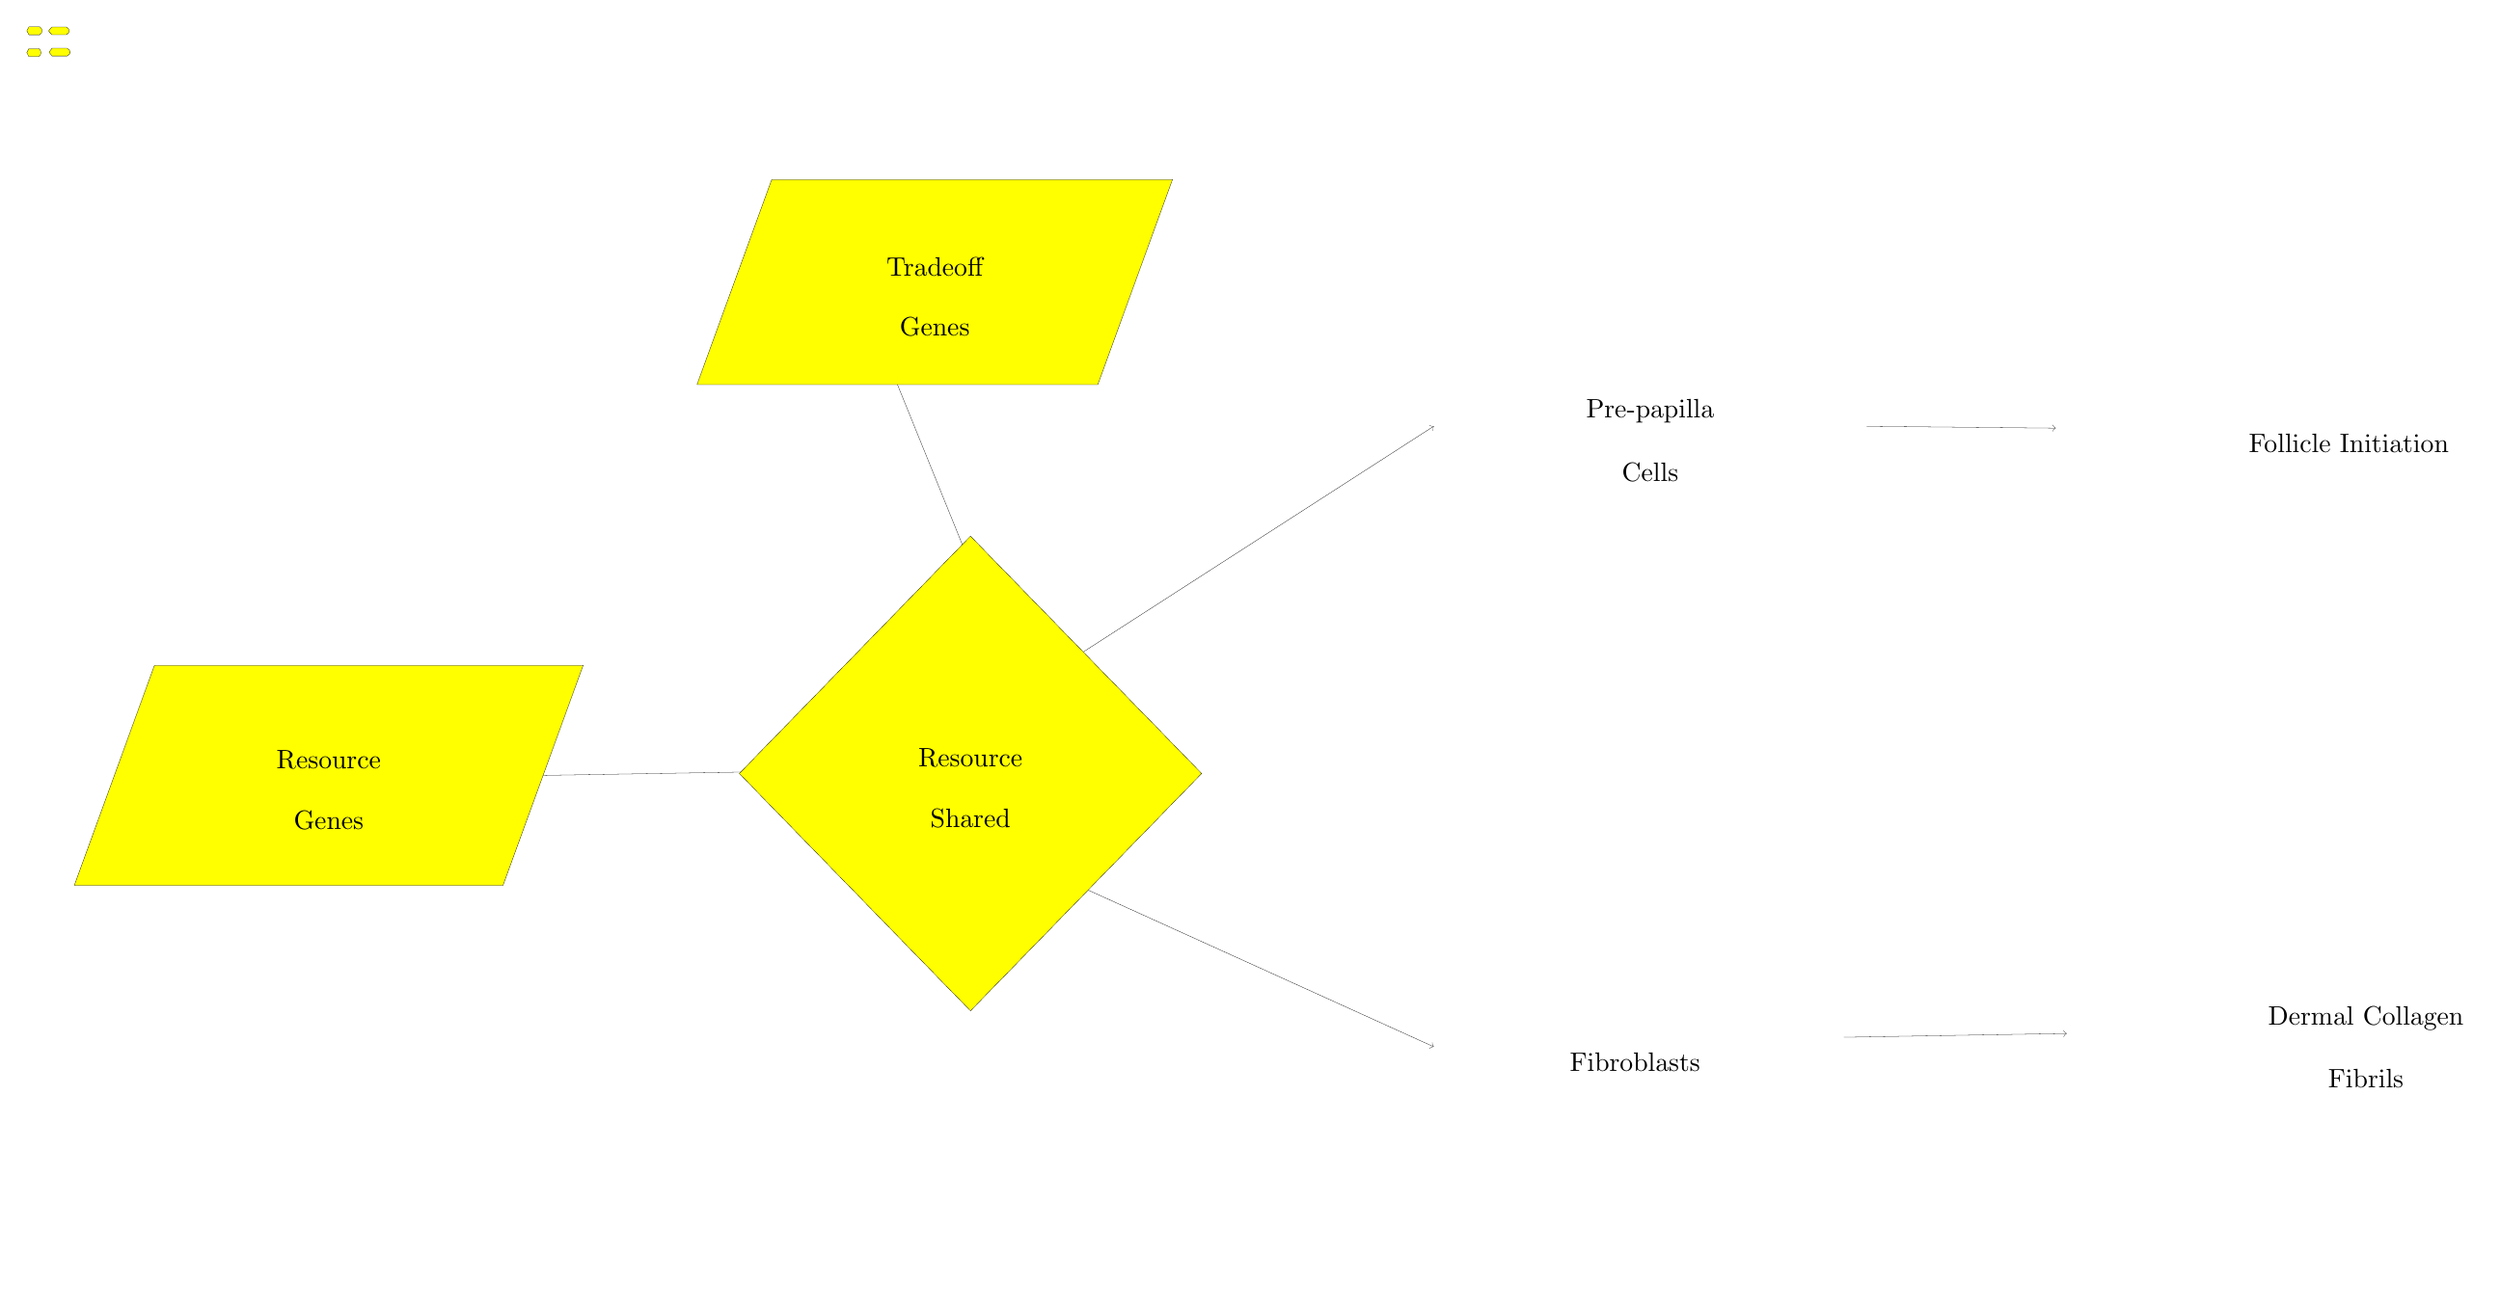
\begin{tikzpicture}
\pgftransformxscale{1.000000}
\pgftransformyscale{-1.000000}
\definecolor{dialinecolor}{rgb}{0.000000, 0.000000, 0.000000}
\pgfsetstrokecolor{dialinecolor}
\definecolor{dialinecolor}{rgb}{1.000000, 1.000000, 1.000000}
\pgfsetfillcolor{dialinecolor}
\pgfsetlinewidth{0.100000\du}
\pgfsetdash{}{0pt}
\pgfsetdash{}{0pt}
\pgfsetbuttcap
\pgfsetmiterjoin
\pgfsetlinewidth{0.100000\du}
\pgfsetbuttcap
\pgfsetmiterjoin
\pgfsetdash{}{0pt}
\definecolor{dialinecolor}{rgb}{1.000000, 1.000000, 0.000000}
\pgfsetfillcolor{dialinecolor}
\fill (13.050000\du,7.100000\du)--(15.650000\du,9.950000\du)--(13.050000\du,12.800000\du)--(10.450000\du,9.950000\du)--cycle;
\definecolor{dialinecolor}{rgb}{0.101961, 0.101961, 0.101961}
\pgfsetstrokecolor{dialinecolor}
\draw (13.050000\du,7.100000\du)--(15.650000\du,9.950000\du)--(13.050000\du,12.800000\du)--(10.450000\du,9.950000\du)--cycle;
\pgfsetbuttcap
\pgfsetmiterjoin
\pgfsetdash{}{0pt}
\definecolor{dialinecolor}{rgb}{0.101961, 0.101961, 0.101961}
\pgfsetstrokecolor{dialinecolor}
\draw (10.450000\du,9.950000\du)--(15.650000\du,9.950000\du);
\definecolor{dialinecolor}{rgb}{1.000000, 1.000000, 0.000000}
\pgfsetfillcolor{dialinecolor}
\fill (2.355514\du,8.550000\du)--(8.000000\du,8.550000\du)--(6.944486\du,11.450000\du)--(1.300000\du,11.450000\du)--cycle;
\pgfsetlinewidth{0.100000\du}
\pgfsetdash{}{0pt}
\pgfsetdash{}{0pt}
\pgfsetmiterjoin
\definecolor{dialinecolor}{rgb}{0.101961, 0.101961, 0.101961}
\pgfsetstrokecolor{dialinecolor}
\draw (2.355514\du,8.550000\du)--(8.000000\du,8.550000\du)--(6.944486\du,11.450000\du)--(1.300000\du,11.450000\du)--cycle;
% setfont left to latex
\definecolor{dialinecolor}{rgb}{0.101961, 0.101961, 0.101961}
\pgfsetstrokecolor{dialinecolor}
\node at (4.650000\du,9.795000\du){Resource};
% setfont left to latex
\definecolor{dialinecolor}{rgb}{0.101961, 0.101961, 0.101961}
\pgfsetstrokecolor{dialinecolor}
\node at (4.650000\du,10.595000\du){Genes};
% setfont left to latex
\definecolor{dialinecolor}{rgb}{0.101961, 0.101961, 0.101961}
\pgfsetstrokecolor{dialinecolor}
\node[anchor=west] at (4.650000\du,10.000000\du){};
% setfont left to latex
\definecolor{dialinecolor}{rgb}{0.101961, 0.101961, 0.101961}
\pgfsetstrokecolor{dialinecolor}
\node[anchor=west] at (4.650000\du,10.000000\du){   };
% setfont left to latex
\definecolor{dialinecolor}{rgb}{0.101961, 0.101961, 0.101961}
\pgfsetstrokecolor{dialinecolor}
\node[anchor=west] at (4.650000\du,10.000000\du){};
% setfont left to latex
\definecolor{dialinecolor}{rgb}{0.101961, 0.101961, 0.101961}
\pgfsetstrokecolor{dialinecolor}
\node[anchor=west] at (4.650000\du,10.000000\du){};
\definecolor{dialinecolor}{rgb}{1.000000, 1.000000, 0.000000}
\pgfsetfillcolor{dialinecolor}
\fill (10.482720\du,2.150000\du)--(15.759558\du,2.150000\du)--(14.776839\du,4.850000\du)--(9.500000\du,4.850000\du)--cycle;
\pgfsetlinewidth{0.100000\du}
\pgfsetdash{}{0pt}
\pgfsetdash{}{0pt}
\pgfsetmiterjoin
\definecolor{dialinecolor}{rgb}{0.101961, 0.101961, 0.101961}
\pgfsetstrokecolor{dialinecolor}
\draw (10.482720\du,2.150000\du)--(15.759558\du,2.150000\du)--(14.776839\du,4.850000\du)--(9.500000\du,4.850000\du)--cycle;
% setfont left to latex
\definecolor{dialinecolor}{rgb}{0.101961, 0.101961, 0.101961}
\pgfsetstrokecolor{dialinecolor}
\node at (12.629779\du,3.295000\du){Tradeoff};
% setfont left to latex
\definecolor{dialinecolor}{rgb}{0.101961, 0.101961, 0.101961}
\pgfsetstrokecolor{dialinecolor}
\node at (12.629779\du,4.095000\du){Genes};
% setfont left to latex
\definecolor{dialinecolor}{rgb}{0.101961, 0.101961, 0.101961}
\pgfsetstrokecolor{dialinecolor}
\node[anchor=west] at (12.629800\du,3.500000\du){};
% setfont left to latex
\definecolor{dialinecolor}{rgb}{0.101961, 0.101961, 0.101961}
\pgfsetstrokecolor{dialinecolor}
\node[anchor=west] at (12.629800\du,3.500000\du){};
% setfont left to latex
\definecolor{dialinecolor}{rgb}{0.101961, 0.101961, 0.101961}
\pgfsetstrokecolor{dialinecolor}
\node[anchor=west] at (12.629800\du,4.300000\du){};
% setfont left to latex
\definecolor{dialinecolor}{rgb}{0.101961, 0.101961, 0.101961}
\pgfsetstrokecolor{dialinecolor}
\node[anchor=west] at (12.629800\du,3.500000\du){};
% setfont left to latex
\definecolor{dialinecolor}{rgb}{0.101961, 0.101961, 0.101961}
\pgfsetstrokecolor{dialinecolor}
\node[anchor=west] at (12.629800\du,3.500000\du){};
% setfont left to latex
\definecolor{dialinecolor}{rgb}{0.101961, 0.101961, 0.101961}
\pgfsetstrokecolor{dialinecolor}
\node[anchor=west] at (12.629800\du,3.500000\du){};
% setfont left to latex
\definecolor{dialinecolor}{rgb}{0.101961, 0.101961, 0.101961}
\pgfsetstrokecolor{dialinecolor}
\node[anchor=west] at (12.629800\du,3.500000\du){};
% setfont left to latex
\definecolor{dialinecolor}{rgb}{0.101961, 0.101961, 0.101961}
\pgfsetstrokecolor{dialinecolor}
\node[anchor=west] at (13.050000\du,9.950000\du){};
% setfont left to latex
\definecolor{dialinecolor}{rgb}{0.101961, 0.101961, 0.101961}
\pgfsetstrokecolor{dialinecolor}
\node[anchor=west] at (13.050000\du,9.950000\du){};
% setfont left to latex
\definecolor{dialinecolor}{rgb}{0.101961, 0.101961, 0.101961}
\pgfsetstrokecolor{dialinecolor}
\node[anchor=west] at (13.050000\du,9.950000\du){};
% setfont left to latex
\definecolor{dialinecolor}{rgb}{0.101961, 0.101961, 0.101961}
\pgfsetstrokecolor{dialinecolor}
\node[anchor=west] at (13.050000\du,9.950000\du){};
% setfont left to latex
\definecolor{dialinecolor}{rgb}{0.101961, 0.101961, 0.101961}
\pgfsetstrokecolor{dialinecolor}
\node[anchor=west] at (5.300000\du,16.550000\du){};
% setfont left to latex
\definecolor{dialinecolor}{rgb}{0.101961, 0.101961, 0.101961}
\pgfsetstrokecolor{dialinecolor}
\node[anchor=west] at (13.050000\du,9.950000\du){};
% setfont left to latex
\definecolor{dialinecolor}{rgb}{0.101961, 0.101961, 0.101961}
\pgfsetstrokecolor{dialinecolor}
\node[anchor=west] at (13.050000\du,9.950000\du){};
% setfont left to latex
\definecolor{dialinecolor}{rgb}{0.101961, 0.101961, 0.101961}
\pgfsetstrokecolor{dialinecolor}
\node[anchor=west] at (13.050000\du,9.950000\du){};
% setfont left to latex
\definecolor{dialinecolor}{rgb}{0.101961, 0.101961, 0.101961}
\pgfsetstrokecolor{dialinecolor}
\node[anchor=west] at (13.050000\du,9.950000\du){};
% setfont left to latex
\definecolor{dialinecolor}{rgb}{0.101961, 0.101961, 0.101961}
\pgfsetstrokecolor{dialinecolor}
\node[anchor=west] at (13.050000\du,9.950000\du){};
% setfont left to latex
\definecolor{dialinecolor}{rgb}{0.101961, 0.101961, 0.101961}
\pgfsetstrokecolor{dialinecolor}
\node[anchor=west] at (11.750000\du,9.800000\du){Resource };
\pgfsetlinewidth{0.100000\du}
\pgfsetdash{}{0pt}
\pgfsetdash{}{0pt}
\pgfsetbuttcap
\pgfsetmiterjoin
\pgfsetlinewidth{0.100000\du}
\pgfsetbuttcap
\pgfsetmiterjoin
\pgfsetdash{}{0pt}
\definecolor{dialinecolor}{rgb}{1.000000, 1.000000, 0.000000}
\pgfsetfillcolor{dialinecolor}
\pgfpathmoveto{\pgfpoint{20.014286\du}{3.900000\du}}
\pgfpathlineto{\pgfpoint{24.085714\du}{3.900000\du}}
\pgfpathcurveto{\pgfpoint{24.696429\du}{4.500000\du}}{\pgfpoint{24.900000\du}{4.800000\du}}{\pgfpoint{24.900000\du}{5.400000\du}}
\pgfpathcurveto{\pgfpoint{24.900000\du}{6.000000\du}}{\pgfpoint{24.696429\du}{6.300000\du}}{\pgfpoint{24.085714\du}{6.900000\du}}
\pgfpathlineto{\pgfpoint{20.014286\du}{6.900000\du}}
\pgfpathlineto{\pgfpoint{19.200000\du}{5.400000\du}}
\pgfpathlineto{\pgfpoint{20.014286\du}{3.900000\du}}
\pgfusepath{fill}
\definecolor{dialinecolor}{rgb}{0.101961, 0.101961, 0.101961}
\pgfsetstrokecolor{dialinecolor}
\pgfpathmoveto{\pgfpoint{20.014286\du}{3.900000\du}}
\pgfpathlineto{\pgfpoint{24.085714\du}{3.900000\du}}
\pgfpathcurveto{\pgfpoint{24.696429\du}{4.500000\du}}{\pgfpoint{24.900000\du}{4.800000\du}}{\pgfpoint{24.900000\du}{5.400000\du}}
\pgfpathcurveto{\pgfpoint{24.900000\du}{6.000000\du}}{\pgfpoint{24.696429\du}{6.300000\du}}{\pgfpoint{24.085714\du}{6.900000\du}}
\pgfpathlineto{\pgfpoint{20.014286\du}{6.900000\du}}
\pgfpathlineto{\pgfpoint{19.200000\du}{5.400000\du}}
\pgfpathlineto{\pgfpoint{20.014286\du}{3.900000\du}}
\pgfusepath{stroke}
% setfont left to latex
\definecolor{dialinecolor}{rgb}{0.101961, 0.101961, 0.101961}
\pgfsetstrokecolor{dialinecolor}
\node at (22.050000\du,5.200000\du){Pre-papilla};
% setfont left to latex
\definecolor{dialinecolor}{rgb}{0.101961, 0.101961, 0.101961}
\pgfsetstrokecolor{dialinecolor}
\node at (22.050000\du,6.000000\du){Cells};
\pgfsetlinewidth{0.100000\du}
\pgfsetdash{}{0pt}
\pgfsetdash{}{0pt}
\pgfsetbuttcap
\pgfsetmiterjoin
\pgfsetlinewidth{0.100000\du}
\pgfsetbuttcap
\pgfsetmiterjoin
\pgfsetdash{}{0pt}
\definecolor{dialinecolor}{rgb}{1.000000, 1.000000, 0.000000}
\pgfsetfillcolor{dialinecolor}
\pgfpathmoveto{\pgfpoint{19.957143\du}{12.100000\du}}
\pgfpathlineto{\pgfpoint{23.742857\du}{12.100000\du}}
\pgfpathcurveto{\pgfpoint{24.310714\du}{12.690000\du}}{\pgfpoint{24.500000\du}{12.985000\du}}{\pgfpoint{24.500000\du}{13.575000\du}}
\pgfpathcurveto{\pgfpoint{24.500000\du}{14.165000\du}}{\pgfpoint{24.310714\du}{14.460000\du}}{\pgfpoint{23.742857\du}{15.050000\du}}
\pgfpathlineto{\pgfpoint{19.957143\du}{15.050000\du}}
\pgfpathlineto{\pgfpoint{19.200000\du}{13.575000\du}}
\pgfpathlineto{\pgfpoint{19.957143\du}{12.100000\du}}
\pgfusepath{fill}
\definecolor{dialinecolor}{rgb}{0.101961, 0.101961, 0.101961}
\pgfsetstrokecolor{dialinecolor}
\pgfpathmoveto{\pgfpoint{19.957143\du}{12.100000\du}}
\pgfpathlineto{\pgfpoint{23.742857\du}{12.100000\du}}
\pgfpathcurveto{\pgfpoint{24.310714\du}{12.690000\du}}{\pgfpoint{24.500000\du}{12.985000\du}}{\pgfpoint{24.500000\du}{13.575000\du}}
\pgfpathcurveto{\pgfpoint{24.500000\du}{14.165000\du}}{\pgfpoint{24.310714\du}{14.460000\du}}{\pgfpoint{23.742857\du}{15.050000\du}}
\pgfpathlineto{\pgfpoint{19.957143\du}{15.050000\du}}
\pgfpathlineto{\pgfpoint{19.200000\du}{13.575000\du}}
\pgfpathlineto{\pgfpoint{19.957143\du}{12.100000\du}}
\pgfusepath{stroke}
% setfont left to latex
\definecolor{dialinecolor}{rgb}{0.101961, 0.101961, 0.101961}
\pgfsetstrokecolor{dialinecolor}
\node at (21.850000\du,13.775000\du){Fibroblasts};
% setfont left to latex
\definecolor{dialinecolor}{rgb}{0.101961, 0.101961, 0.101961}
\pgfsetstrokecolor{dialinecolor}
\node[anchor=west] at (22.864300\du,5.400000\du){};
% setfont left to latex
\definecolor{dialinecolor}{rgb}{0.101961, 0.101961, 0.101961}
\pgfsetstrokecolor{dialinecolor}
\node[anchor=west] at (22.607100\du,13.575000\du){};
\pgfsetlinewidth{0.100000\du}
\pgfsetdash{}{0pt}
\pgfsetdash{}{0pt}
\pgfsetbuttcap
\pgfsetmiterjoin
\pgfsetlinewidth{0.100000\du}
\pgfsetbuttcap
\pgfsetmiterjoin
\pgfsetdash{}{0pt}
\definecolor{dialinecolor}{rgb}{1.000000, 1.000000, 0.000000}
\pgfsetfillcolor{dialinecolor}
\pgfpathmoveto{\pgfpoint{28.492500\du}{4.000000\du}}
\pgfpathlineto{\pgfpoint{34.007500\du}{4.000000\du}}
\pgfpathcurveto{\pgfpoint{34.834750\du}{4.570000\du}}{\pgfpoint{35.110500\du}{4.855000\du}}{\pgfpoint{35.110500\du}{5.425000\du}}
\pgfpathcurveto{\pgfpoint{35.110500\du}{5.995000\du}}{\pgfpoint{34.834750\du}{6.280000\du}}{\pgfpoint{34.007500\du}{6.850000\du}}
\pgfpathlineto{\pgfpoint{28.492500\du}{6.850000\du}}
\pgfpathlineto{\pgfpoint{27.389500\du}{5.425000\du}}
\pgfpathlineto{\pgfpoint{28.492500\du}{4.000000\du}}
\pgfusepath{fill}
\definecolor{dialinecolor}{rgb}{0.101961, 0.101961, 0.101961}
\pgfsetstrokecolor{dialinecolor}
\pgfpathmoveto{\pgfpoint{28.492500\du}{4.000000\du}}
\pgfpathlineto{\pgfpoint{34.007500\du}{4.000000\du}}
\pgfpathcurveto{\pgfpoint{34.834750\du}{4.570000\du}}{\pgfpoint{35.110500\du}{4.855000\du}}{\pgfpoint{35.110500\du}{5.425000\du}}
\pgfpathcurveto{\pgfpoint{35.110500\du}{5.995000\du}}{\pgfpoint{34.834750\du}{6.280000\du}}{\pgfpoint{34.007500\du}{6.850000\du}}
\pgfpathlineto{\pgfpoint{28.492500\du}{6.850000\du}}
\pgfpathlineto{\pgfpoint{27.389500\du}{5.425000\du}}
\pgfpathlineto{\pgfpoint{28.492500\du}{4.000000\du}}
\pgfusepath{stroke}
% setfont left to latex
\definecolor{dialinecolor}{rgb}{0.101961, 0.101961, 0.101961}
\pgfsetstrokecolor{dialinecolor}
\node at (31.250000\du,5.625000\du){Follicle Initiation};
\pgfsetlinewidth{0.100000\du}
\pgfsetdash{}{0pt}
\pgfsetdash{}{0pt}
\pgfsetbuttcap
\pgfsetmiterjoin
\pgfsetlinewidth{0.100000\du}
\pgfsetbuttcap
\pgfsetmiterjoin
\pgfsetdash{}{0pt}
\definecolor{dialinecolor}{rgb}{1.000000, 1.000000, 0.000000}
\pgfsetfillcolor{dialinecolor}
\pgfpathmoveto{\pgfpoint{28.660000\du}{11.950000\du}}
\pgfpathlineto{\pgfpoint{34.290000\du}{11.950000\du}}
\pgfpathcurveto{\pgfpoint{35.134500\du}{12.530000\du}}{\pgfpoint{35.416000\du}{12.820000\du}}{\pgfpoint{35.416000\du}{13.400000\du}}
\pgfpathcurveto{\pgfpoint{35.416000\du}{13.980000\du}}{\pgfpoint{35.134500\du}{14.270000\du}}{\pgfpoint{34.290000\du}{14.850000\du}}
\pgfpathlineto{\pgfpoint{28.660000\du}{14.850000\du}}
\pgfpathlineto{\pgfpoint{27.534000\du}{13.400000\du}}
\pgfpathlineto{\pgfpoint{28.660000\du}{11.950000\du}}
\pgfusepath{fill}
\definecolor{dialinecolor}{rgb}{0.101961, 0.101961, 0.101961}
\pgfsetstrokecolor{dialinecolor}
\pgfpathmoveto{\pgfpoint{28.660000\du}{11.950000\du}}
\pgfpathlineto{\pgfpoint{34.290000\du}{11.950000\du}}
\pgfpathcurveto{\pgfpoint{35.134500\du}{12.530000\du}}{\pgfpoint{35.416000\du}{12.820000\du}}{\pgfpoint{35.416000\du}{13.400000\du}}
\pgfpathcurveto{\pgfpoint{35.416000\du}{13.980000\du}}{\pgfpoint{35.134500\du}{14.270000\du}}{\pgfpoint{34.290000\du}{14.850000\du}}
\pgfpathlineto{\pgfpoint{28.660000\du}{14.850000\du}}
\pgfpathlineto{\pgfpoint{27.534000\du}{13.400000\du}}
\pgfpathlineto{\pgfpoint{28.660000\du}{11.950000\du}}
\pgfusepath{stroke}
% setfont left to latex
\definecolor{dialinecolor}{rgb}{0.101961, 0.101961, 0.101961}
\pgfsetstrokecolor{dialinecolor}
\node at (31.475000\du,13.200000\du){Dermal Collagen};
% setfont left to latex
\definecolor{dialinecolor}{rgb}{0.101961, 0.101961, 0.101961}
\pgfsetstrokecolor{dialinecolor}
\node at (31.475000\du,14.000000\du){Fibrils};
% setfont left to latex
\definecolor{dialinecolor}{rgb}{0.101961, 0.101961, 0.101961}
\pgfsetstrokecolor{dialinecolor}
\node[anchor=west] at (32.353000\du,5.425000\du){};
% setfont left to latex
\definecolor{dialinecolor}{rgb}{0.101961, 0.101961, 0.101961}
\pgfsetstrokecolor{dialinecolor}
\node[anchor=west] at (32.601000\du,13.400000\du){};
\pgfsetlinewidth{0.100000\du}
\pgfsetdash{}{0pt}
\pgfsetdash{}{0pt}
\pgfsetbuttcap
{
\definecolor{dialinecolor}{rgb}{0.101961, 0.101961, 0.101961}
\pgfsetfillcolor{dialinecolor}
% was here!!!
\pgfsetarrowsend{to}
\definecolor{dialinecolor}{rgb}{0.101961, 0.101961, 0.101961}
\pgfsetstrokecolor{dialinecolor}
\draw (7.472240\du,10.000000\du)--(10.450000\du,9.950000\du);
}
\pgfsetlinewidth{0.100000\du}
\pgfsetdash{}{0pt}
\pgfsetdash{}{0pt}
\pgfsetbuttcap
{
\definecolor{dialinecolor}{rgb}{0.101961, 0.101961, 0.101961}
\pgfsetfillcolor{dialinecolor}
% was here!!!
\pgfsetarrowsend{to}
\definecolor{dialinecolor}{rgb}{0.101961, 0.101961, 0.101961}
\pgfsetstrokecolor{dialinecolor}
\draw (12.138400\du,4.850000\du)--(13.050000\du,7.100000\du);
}
\pgfsetlinewidth{0.100000\du}
\pgfsetdash{}{0pt}
\pgfsetdash{}{0pt}
\pgfsetbuttcap
{
\definecolor{dialinecolor}{rgb}{0.101961, 0.101961, 0.101961}
\pgfsetfillcolor{dialinecolor}
% was here!!!
\pgfsetarrowsend{to}
\definecolor{dialinecolor}{rgb}{0.101961, 0.101961, 0.101961}
\pgfsetstrokecolor{dialinecolor}
\draw (14.350000\du,8.525000\du)--(19.200000\du,5.400000\du);
}
\pgfsetlinewidth{0.100000\du}
\pgfsetdash{}{0pt}
\pgfsetdash{}{0pt}
\pgfsetbuttcap
{
\definecolor{dialinecolor}{rgb}{0.101961, 0.101961, 0.101961}
\pgfsetfillcolor{dialinecolor}
% was here!!!
\pgfsetarrowsend{to}
\definecolor{dialinecolor}{rgb}{0.101961, 0.101961, 0.101961}
\pgfsetstrokecolor{dialinecolor}
\draw (14.350000\du,11.375000\du)--(19.200000\du,13.575000\du);
}
\pgfsetlinewidth{0.100000\du}
\pgfsetdash{}{0pt}
\pgfsetdash{}{0pt}
\pgfsetbuttcap
{
\definecolor{dialinecolor}{rgb}{0.101961, 0.101961, 0.101961}
\pgfsetfillcolor{dialinecolor}
% was here!!!
\pgfsetarrowsend{to}
\definecolor{dialinecolor}{rgb}{0.101961, 0.101961, 0.101961}
\pgfsetstrokecolor{dialinecolor}
\draw (24.900000\du,5.400000\du)--(27.389500\du,5.425000\du);
}
\pgfsetlinewidth{0.100000\du}
\pgfsetdash{}{0pt}
\pgfsetdash{}{0pt}
\pgfsetbuttcap
{
\definecolor{dialinecolor}{rgb}{0.101961, 0.101961, 0.101961}
\pgfsetfillcolor{dialinecolor}
% was here!!!
\pgfsetarrowsend{to}
\definecolor{dialinecolor}{rgb}{0.101961, 0.101961, 0.101961}
\pgfsetstrokecolor{dialinecolor}
\draw (24.600000\du,13.450000\du)--(27.534000\du,13.400000\du);
}
\definecolor{dialinecolor}{rgb}{1.000000, 1.000000, 0.000000}
\pgfsetfillcolor{dialinecolor}
\fill (13.100000\du,6.848080\du)--(16.143904\du,9.975000\du)--(13.100000\du,13.101920\du)--(10.056096\du,9.975000\du)--cycle;
\pgfsetlinewidth{0.100000\du}
\pgfsetdash{}{0pt}
\pgfsetdash{}{0pt}
\pgfsetmiterjoin
\definecolor{dialinecolor}{rgb}{0.101961, 0.101961, 0.101961}
\pgfsetstrokecolor{dialinecolor}
\draw (13.100000\du,6.848080\du)--(16.143904\du,9.975000\du)--(13.100000\du,13.101920\du)--(10.056096\du,9.975000\du)--cycle;
% setfont left to latex
\definecolor{dialinecolor}{rgb}{0.101961, 0.101961, 0.101961}
\pgfsetstrokecolor{dialinecolor}
\node at (13.100000\du,9.770000\du){Resource};
% setfont left to latex
\definecolor{dialinecolor}{rgb}{0.101961, 0.101961, 0.101961}
\pgfsetstrokecolor{dialinecolor}
\node at (13.100000\du,10.570000\du){Shared};
% setfont left to latex
\definecolor{dialinecolor}{rgb}{0.101961, 0.101961, 0.101961}
\pgfsetstrokecolor{dialinecolor}
\node[anchor=west] at (13.100000\du,9.975000\du){};
\end{tikzpicture}
  \caption{Diagram of the postulated tradeoff relationship between pre-papilla cell differentiation and fibroblast differerentiation}
\end{figure}
\end{landscape}
%\end{document}

